\documentclass[11pt,letterpaper]{article}

\usepackage{eso-pic}

\AddToShipoutPictureBG{%

\ifnum\value{page}>1{
\AtTextUpperLeft{
\makebox[\textwidth][r]{
\raisebox{-1.3cm}{%
{\transparent{0.3}{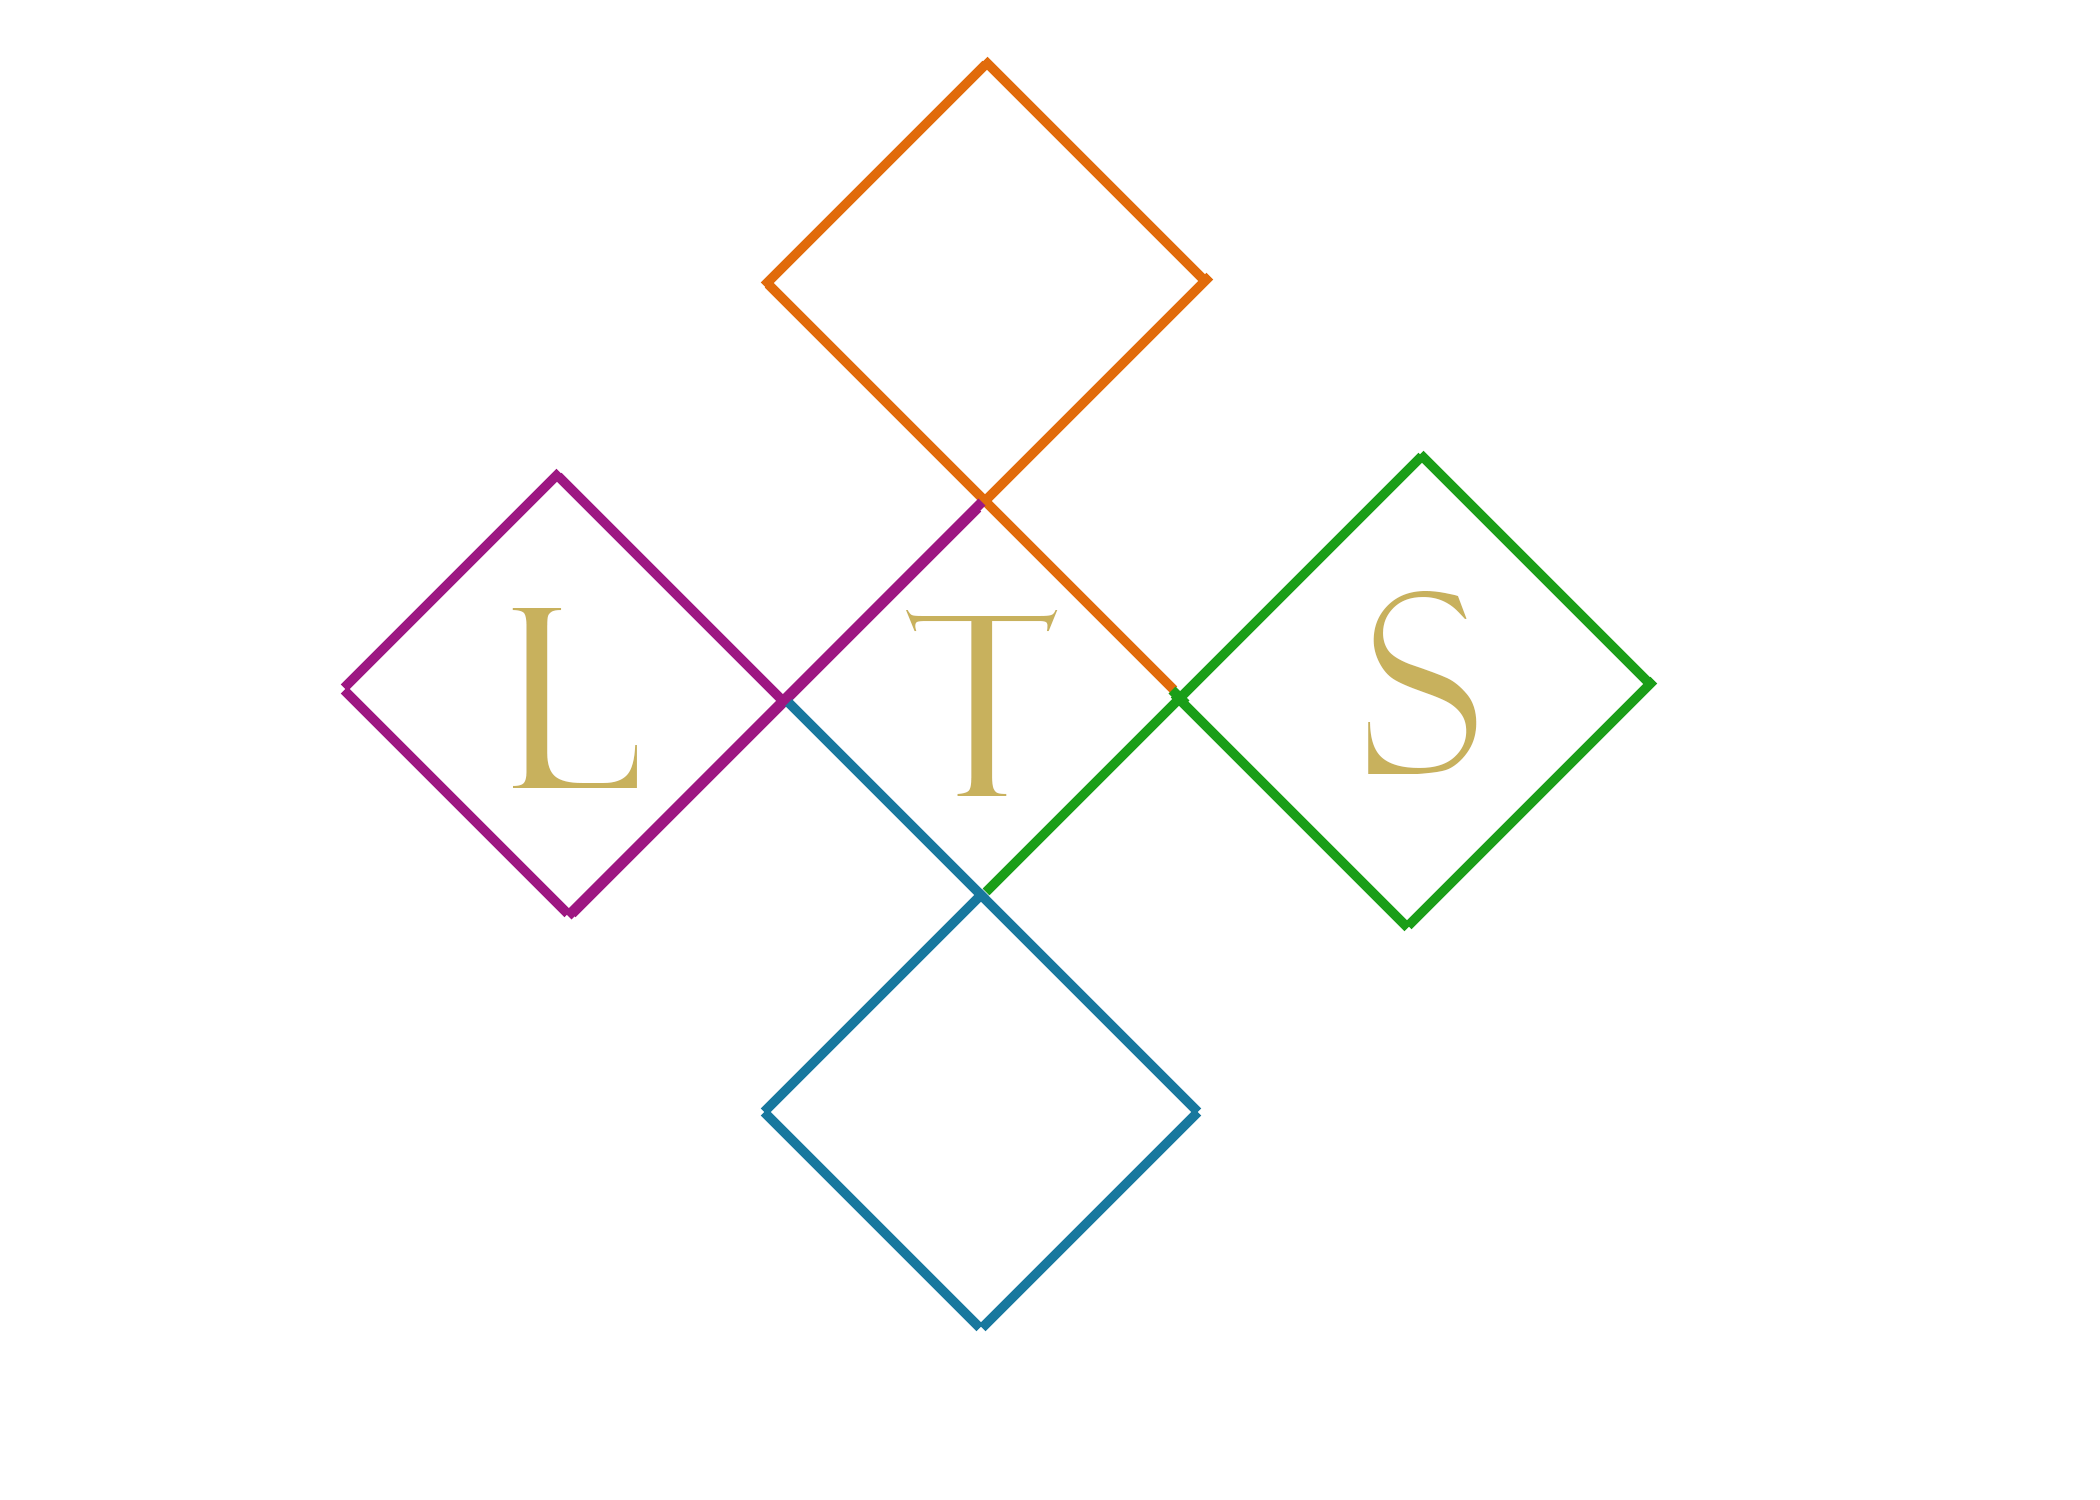
\includegraphics[width=0.25\textwidth]{e-logo.png}}	}} } }
}\fi
}


\AddToShipoutPicture{%
{
 {\color{blGreen!70!red}\transparent{0.9}{\put(0,0){\rule{.55cm}{\paperheight}}}}%
 {\color{darkRed!70!purple}\transparent{1}\put(6,0){{\rule{.3cm}{\paperheight}}}}
 \ifnum\value{page}>3{ 
 {\color{logoPeach!80!cyan}\transparent{0.5}{\put(0,760){\rule{1cm}{.6cm}}}}%
 {\color{darkRed!60!cyan}\transparent{0.7}\put(0,766){{\rule{1cm}{.6cm}}}}
 \put(8,786){\thepage}
 \transparent{0.8}}\fi
}
}

%\put(0,4){%
%\transparent{1}{
%
\includegraphics[width=0.1\textwidth]{logo.jpg}} }




\AddToShipoutPicture{%

\ifnum\value{page}>0


{\color{blGreen!70!red}\transparent{0.9}{\put(300,12){\rule{0.5\paperwidth}{.3cm}}}}%
{\color{inOne}\transparent{0.8}{\put(300,15){\rule{0.5\paperwidth}{.3cm}}}}%
{\color{inTwo}\transparent{0.3}\put(300,18){{\rule{0.5\paperwidth}{.3cm}}}}

\put(470,12){%
\transparent{0.7}{

\includegraphics[width=0.2\textwidth]{logo.png}} }

{\color{blGreen!70!red}\transparent{0.9}{\put(5.6,10){\rule{0.5\paperwidth}{.4cm}}}}%
{\color{inOne}\transparent{1}{\put(5.6,15){\rule{0.5\paperwidth}{.4cm}}}}%
{\color{inTwo}\transparent{0.3}\put(5.6,20){{\rule{0.5\paperwidth}{.4cm}}}}

\fi
}


%\pagestyle{empty} % no page number
%\parskip 7.2pt    % space between paragraphs
%\parindent 12pt   % indent for new paragraph
%\textwidth 4.5in  % width of text
%\columnsep 0.8in  % separation between columns

\usepackage{geometry}
\geometry{left=.85in,top=.85in,right=.5in,bottom=1.1in} %margins
\usepackage{graphicx}
\usepackage{color,framed}

\usepackage{float}

\usepackage{mdframed}


\usepackage{setspace}
\newcommand{\rpdfNotice}[1]{\begin{onehalfspacing}{

\Large #1

}\end{onehalfspacing}}

\usepackage{xcolor}

\usepackage[hyphenbreaks]{breakurl}
\usepackage[hyphens]{url}

\usepackage{hyperref}
\newcommand{\rpdfLink}[1]{\href{#1}{\small{#1}}}
\newcommand{\dblHref}[1]{\href{#1}{\small{\burl{#1}}}}
\newcommand{\browseHref}[2]{\href{#1}{\Large #2}}

\hypersetup{
    colorlinks=true,
    linkcolor=cyan,
    filecolor=magenta,
    urlcolor=blue,
}

\urlstyle{same}

\definecolor{blGreen}{rgb}{.2,.7,.3}
\definecolor{darkRed}{rgb}{.2,.0,.1}

\definecolor{darkBlGreen}{rgb}{.1,.3,.2}

\definecolor{oldBlColor}{rgb}{.2,.7,.3}

\definecolor{blColor}{rgb}{.1,.3,.2}

\definecolor{elColor}{rgb}{.2,.1,0}
\definecolor{flColor}{rgb}{0.7,0.3,0.3}

\definecolor{logoOrange}{RGB}{108, 18, 30}
\definecolor{logoGreen}{RGB}{85, 153, 89}
\definecolor{logoPurple}{RGB}{200, 208, 30}

\definecolor{logoBlue}{RGB}{4, 2, 25}
\definecolor{logoPeach}{RGB}{255, 159, 102}
\definecolor{logoCyan}{RGB}{66, 206, 244}
\definecolor{logoRed}{rgb}{.3,0,0}

\definecolor{inOne}{rgb}{0.122, 0.435, 0.698}% Rule colour
\definecolor{inTwo}{rgb}{0.122, 0.698, 0.435}% Rule colour

\definecolor{outOne}{rgb}{0.435, 0.698, 0.122}% Rule colour
\definecolor{outTwo}{rgb}{0.698, 0.435, 0.122}% Rule colour

\usepackage{tcolorbox}% http://ctan.org/pkg/tcolorbox

\usepackage{transparent}

\newenvironment{cframed}{\begin{mdframed}[linecolor=logoPeach,linewidth=0.4mm]}{\end{mdframed}}

\newenvironment{ccframed}{\begin{mdframed}[backgroundcolor=logoGreen!5,linecolor=logoCyan!50!black,linewidth=0.4mm]}{\end{mdframed}}

\usepackage{aurical}
\usepackage[T1]{fontenc}

\usepackage{relsize}

\newcommand{\YPDFI}{{\fontfamily{fvs}\selectfont YPDF-Interactive}}

%
\newcommand{\deconum}[1]{{\protect\raisebox{-1pt}{{\LARGE #1}}}}

%\newcommand{\deconum}[1]{{\textcircled{#1}}}


\renewcommand{\thesection}{\protect\mbox{\deconum{\Roman{section}}}}
\renewcommand{\thesubsection}{\arabic{section}.\arabic{subsection}}


%\usepackage{sectsty}
\usepackage{titlesec}
\usepackage{url}

\usepackage{eso-pic}

\usepackage{setspace}
%\doublespacing
%\onehalfspacing


% line
\usepackage[object=vectorian]{pgfornament} %%  http://altermundus.com/pages/tkz/ornament/index.html

\definecolor{darkRed}{rgb}{.2,.0,.1}

\newcommand{\decoline}{%

\vspace{-2em}
{\color{darkRed!60!cyan}\noindent\hfil{\EnglischeLinie}\hfil}
%{\color{darkRed!60!cyan}\noindent\hfil\rule{0.5\textwidth}{.8pt}\hfil}
\vspace{-2.25em}}


\newcommand{\whdecoline}{%

\vspace{-2em}
{\color{white}\noindent\hfil{\whEnglischeLinie}\hfil}
%{\color{darkRed!60!cyan}\noindent\hfil\rule{0.5\textwidth}{.8pt}\hfil}
\vspace{-2.25em}}

\newcommand{\sectionline}[1]{%
  \noindent
  \begin{center}
  {\color{#1}
    \resizebox{0.5\linewidth}{1ex}
    {{%
    {\begin{tikzpicture}
    \node  (C) at (0,0) {};
    \node (D) at (9,0) {};
    \path (C) to [ornament=84] (D);
    \end{tikzpicture}}}}}%
    \end{center}
  }
  
\newcommand{\EnglischeLinie}{
\sectionline{darkRed!60!cyan}
}

\newcommand{\whEnglischeLinie}{
\sectionline{white}
}
% ///


\newcommand{\sectionlinenoc}[2]{%
	\noindent
		{\color{#1}
			\resizebox{#2}{1ex}
			{{%
					{\begin{tikzpicture}
						\node  (C) at (0,0) {};
						\node (D) at (9,0) {};
						\path (C) to [ornament=84] (D);
						\end{tikzpicture}}}}}%
}

\newcommand{\shortsectionline}[1]{%
	\noindent
	\begin{center}
		{\color{#1}
			\resizebox{.2\linewidth}{1.5ex}
			{{%
					{\begin{tikzpicture}
						\node  (C) at (0,0) {};
						\node (D) at (9,0) {};
						\path (C) to [ornament=84] (D);
						\end{tikzpicture}}}}}%
	\end{center}
}

\definecolor{blGreen}{rgb}{.2,.7,.3}

\newcommand{\shortdecoline}{\vspace*{-.65em}\shortsectionline{blGreen!10!orange}\vspace*{-.85em}}
\newcommand{\shortdecolineadj}[2]{\vspace*{#1}\shortsectionline{blGreen!10!orange}\vspace*{#2}}


\usepackage[flushmargin]{footmisc}

\usepackage[letterpaper, left=.45in,right=.45in,top=1in,bottom=1in]{geometry}

\colorlet{codegr}{black!80!blue}

\setlength{\columnsep}{7mm}

%% rightx
\newcommand{\htwoo}{H$_2$O}
\newcommand{\dtwoo}{D$_2$O}
\newcommand{\POne}{$P_1$}
\newcommand{\PTwo}{$P_2$}
\newcommand{\Pone}{$P_1$}
\newcommand{\Ptwo}{$P_2$}
\newcommand{\Pprop}{$P$}

\newcommand{\Stwo}{$S_2$}
\newcommand{\Sone}{$S_1$}

\newcommand{\facondeparler}{\textit{fa{\c{c}}on de parler}}

\newcounter{sentenceCounter}{}

\newcommand{\writeIncSentenceCounter}{\refstepcounter{sentenceCounter}(\arabic{sentenceCounter})}{}


\newcommand{\listItemMark}{\rotatebox{30}{\raisebox{2pt}{\color{green!30!yellow!40!black}{\begin{tiny}$\blacktriangleright$\end{tiny}}}}}
\newenvironment{sentenceList}{\begin{list}{\listItemMark}{\setlength{\leftmargin}{.5em}\setlength{\itemsep}{-.1em}\setlength{\topsep}{.85em}}\begin{small}}{\end{small}\end{list}}

\newcommand{\sentenceItem}{\item \writeIncSentenceCounter}{}
% ///

\usepackage{etoolbox}

\AtBeginEnvironment{thebibliography}{\linespread{1}\selectfont}

%?\usepackage{mathptmx}


%?\titleformat*{\subsection}{\small\bfseries}

%?\usepackage{eufrak}
\usepackage{wasysym}
\usepackage{textcomp}
\usepackage{amssymb}

\usepackage{microtype}



\DeclareMathAlphabet{\mathcal}{OMS}{cmsy}{m}{n}
%\usepackage{euler}

\let\OldI\i


\newcommand{\mdash}{---}
\newcommand{\q}[1]{``#1"}
\newcommand{\sq}[1]{`#1'}
\renewcommand{\i}[1]{\textit{#1}}

\newcommand{\T}[1]{\raisebox{-2pt}{\ensuremath{\mathcal{T}}}\textit{\tiny #1}}
%\newcommand{\T}{\ensuremath{\mathscr{T2}}}

\newcommand{\TSupT}{\ensuremath{{\T2}\makebox[4pt][r]{\raisebox{5pt}{{\scalebox{.6}{\T1}}}}}}

\let\OldFootnoteSize\footnotesize
\renewcommand{\footnotesize}{\scriptsize}
	
%\newcommand{\Tnoindex}{\raisebox{-2pt}{\ensuremath{\mathfrak{t}}}}
\newcommand{\Tnoindex}{\ensuremath{\mathfrak{t}}}

\newcommand{\typeAbove}{%
\raisebox{-1pt}{\rotatebox{90}{\begin{tiny}$\diagdown$\makebox[1pt][c]{$\diagup$}\end{tiny}}}}

%\newcommand{\typeT}{\ensuremath{type\raisebox{.5pt}{\makebox[3pt][c]{-}}T}}
%\newcommand{\typeT}{\ensuremath{\mathcal{T}}}
\newcommand{\typeT}{\ensuremath{\mathfrak{t}}}

\newcommand{\TValues}{\typeT{}-values} 

\newcommand{\emigres}{\'emigr\'es}

\newcommand{\Retore}{Retor\'e}
\newcommand{\Aurelie}{Aur\'elie}
\newcommand{\Descles}{D\'escles}

\newcommand{\ala}{\`a la}

\newcommand{\picalculus}{\ensuremath{\pi}-calculus}

\newcommand{\qmarkdubious}{\raisebox{4pt}{{\footnotesize\textbf{?}}}}

%\newcommand{\TypeCat}{\ensuremath{\mathcal{T}}}
\newcommand{\TypeCat}{\ensuremath{\mathfrak{t}}}

\newcommand{\ADJplusNPeqNP}{\ensuremath{ADJ + NP = NP}}

%\newcommand{\outarrow}{\ensuremath{\overset{..}{\rightarrow}}}

\newcommand{\outarrow}{\makebox[-2pt][l]{%
\raisebox{4pt}{..}}\ensuremath{\rightarrow}}

\newcommand{\argarrow}{\hspace{1pt} \makebox[-2pt][l]{%
		\raisebox{4pt}{.}}\ensuremath{\rightarrow} \hspace{1pt}}


\newcommand{\smoutarrow}{\makebox[-1pt][l]{%
		\raisebox{3pt}{..}}\ensuremath{\rightarrow}}

\newcommand{\smargarrow}{\hspace{1pt} \makebox[-2pt][l]{%
		\raisebox{3pt}{.}}\ensuremath{\rightarrow} \hspace{1pt}}



%\newcommand{\NounToNoun}{N \outarrow N}
%\newcommand{\VisNtoS}{V :: N \outarrow N}

\newcommand{\mmbox}[1]{#1}

\newcommand{\NtoN}{\mmbox{\ensuremath{N} \outarrow{} \ensuremath{N}}}
\newcommand{\NounToNoun}{\mmbox{\ensuremath{N} \outarrow{} \ensuremath{N}}}
\newcommand{\VisNtoS}{\mmbox{\ensuremath{V :: N} \outarrow{} \Prop}}
\newcommand{\AdjisNtoN}{\mmbox{\hspace{2pt}\ensuremath{\mathcal{A}
\scalebox{.7}{\ensuremath{\mathcal{DJ}}} :: N} \outarrow{} \Prop}}


\newcommand{\thatPhrase}{\AcronymText{that}-phrase}
\newcommand{\thatPhrases}{\AcronymText{that}-phrases}

\usepackage{graphicx}

\newcommand{\rzauthor}[3]{{
{\vspace{-4em}}{\fontfamily{gar}\fontseries{b}\selectfont% 
{\begin{center}\textls*[103]{#1}\\ \vspace{-2em}%
{\scalebox{.7}{\fontfamily{phv}\fontshape{it}\selectfont\footnotesize #3}}#2\end{center}}

{\vspace{-2.25em}}
{\hfill\small\today}

{\vspace{.25em}}
}}}			 


\newcommand{\rzauth}[3]{{
		{\vspace{-1em}}{\fontfamily{gar}\fontseries{b}\selectfont% 
			{\begin{center}\textls*[103]{#1}\\ \vspace{1em}%
					{\scalebox{.7}{\fontfamily{phv}\fontshape{it}\selectfont\footnotesize #3}}#2\end{center}}
			
			{\vspace{-6em}}
			{\hfill\small {\raisebox{1em}{\today}}}
			
			{\vspace{0em}}
		}}}			 




\newcommand{\rztitle}[1]{\begin{center}\fontfamily{phv}\fontseries{b}\selectfont #1\end{center}}


\newcommand{\Jorgen}{J{\o}rgen}

\newcommand{\Prop}{\ensuremath{\mathcal{P}rop}}

\newcommand{\NN}{\ensuremath{N}\hspace{-1pt}\argarrow\hspace{-1pt}\ensuremath{N}}
\newcommand{\Npl}{%
\ensuremath{N}\raisebox{8pt}{\hspace{-1pt}\ensuremath{\rotatebox{180}{{\begin{footnotesize}$\dotplus$\end{footnotesize}}}}}}
\newcommand{\NPl}{\Npl}
\newcommand{\NtoNpl}{%
\mmbox{\ensuremath{N} \outarrow{} \Npl}}
\newcommand{\NpltoNpl}{\mmbox{\Npl{} \outarrow{} \Npl}}
\newcommand{\PropToN}{\mmbox{\Prop \hspace{1pt} \outarrow{} \N}}

\newcommand{\VisNNtoProp}{\mmbox{\ensuremath{V :: N} \argarrow \ensuremath{N} \outarrow{} \Prop}}
\newcommand{\VisNProptoProp}{\mmbox{\ensuremath{V :: N} \argarrow  \Prop{} \hspace{2pt} \outarrow{} \Prop}}


\newcommand{\NSing}{\ensuremath{N}\raisebox{5pt}{\scalebox{0.65}{\ensuremath{%
{\odot}}}}}


\newcommand{\Z}{\ensuremath{\mathbb{Z}}}

\newcommand{\VPpNPeqS}{\ensuremath{VP + NP = S}}
\newcommand{\NSingToNPl}{\mmbox{\NSing{} \outarrow{} \Npl}}

\newcommand{\NNtoS}{\mmbox{\NN{} \outarrow{} \Prop}}
\newcommand{\NNtoN}{\mmbox{\NN{} \outarrow{} \ensuremath{N}}}
\newcommand{\N}{\mmbox{\ensuremath{N}}}
\newcommand{\NtoProp}{\mmbox{\N{} \outarrow{} \Prop}}
\newcommand{\NNtoProp}{\mmbox{\NN{} \outarrow{} \Prop{}}}
\newcommand{\ProptoN}{\mmbox{\Prop{} \outarrow{} \N}}


\newcommand{\PropToNYieldsN}{\PropToN{} \raisebox{1pt}{\ensuremath{\textgreater\hspace{-5pt}\raisebox{.15pt}{\ensuremath{\Rightarrow}}}}{} \N}

\newcommand{\SeqNPplVP}{\mmbox{{\small\texttt{S = NP + VP}}}}

\newcommand{\Arg}{\ensuremath{A}\tiny{rg}}
\newcommand{\argsToReturn}{\mbox{\ensuremath{{\Arg}_0} \hspace{-4pt} \smargarrow 
		\hspace{-3pt}
\ensuremath{{\Arg}_1} 
\hspace{-4pt} \smargarrow \hspace{-2pt} \ensuremath{\cdot\cdot\cdot} \hspace{0pt} \smoutarrow  \hspace{1pt} \textit{Result}}}

\newcommand{\lowBlank}{\raisebox{-1pt}{\textthreequartersemdash\textthreequartersemdash\textthreequartersemdash}}

\newcommand{\BlankAfterBlank}{\lowBlank\texttt{after}\lowBlank}
\newcommand{\AfterNSingAndNSingToNPl}{\mbox{\texttt{after} :: %
\NSing \argarrow \NSing \hspace{1pt} \outarrow \hspace{1pt} \Npl}}

\newcommand{\archiveDate}[1]{{\footnotesize #1}}

\newcommand{\sentenceexample}[1]{
\begin{noindent}
\hspace*{-8pt}{{\raisebox{2pt}{{\scriptsize {\color{green!30!yellow!40!black}  
\rotatebox{20}{\RIGHTarrow}}}}} \hspace*{-2pt} #1
	
}
\end{noindent}
}

\newcommand{\sentenceexamples}[1]{
	
\vspace{1em}		
{\setstretch{1.0}	
#1
}
\vspace{.7em}		

\noindent\hspace{-4pt}}



\newcommand{\FeqMtimesA}{\hspace{-2pt}{\small \ensuremath{F}=\ensuremath{M}{\texttimes}\ensuremath{A}}}
\newcommand{\piCalculus}{\ensuremath{\pi}-calculus}


\newif\iffootnote
\let\Footnote\footnote
\renewcommand\footnote[1]{\begingroup\footnotetrue\Footnote{#1}\endgroup}

\newcommand{\AcronymText}[1]{{\iffootnote\begin{footnotesize}{\textsc{#1}}\end{footnotesize}%
\else\begin{OldFootnoteSize}{\textsc{#1}}\end{OldFootnoteSize}\fi}}


\newcommand{\NLP}{\AcronymText{NLP}}
\newcommand{\POS}{\AcronymText{POS}}

\newcommand{\Gardenfors}{G\"ardenfors}


\newcommand{\Haskell}{\AcronymText{Haskell}}
\newcommand{\C}{\AcronymText{C}}
\newcommand{\NP}{\AcronymText{NP}}
\newcommand{\Cpp}{\AcronymText{C++}}
\newcommand{\RDF}{\AcronymText{RDF}}
\newcommand{\Java}{\AcronymText{Java}}
\newcommand{\IT}{\AcronymText{IT}}
\newcommand{\IBMinc}{\AcronymText{IBM}}
\newcommand{\XDG}{\AcronymText{XDG}}
\newcommand{\AI}{\AcronymText{AI}}

\newcommand{\HPSG}{\AcronymText{HPSG}}
\newcommand{\CAG}{\AcronymText{CAG}}
\newcommand{\Lisp}{\AcronymText{Lisp}}

\newcommand{\TS}{\AcronymText{TS}}

\newcommand{\ThreeD}{\AcronymText{3D}}

%?\usepackage[inline]{enumitem}
\usepackage{enumitem}




\usepackage[font=small,labelfont=bf]{caption}

\usepackage{xcolor}

\definecolor{Bkg}{RGB}{250,245,252}
\newcommand{\leader}[2]{\hspace{#1}\colorbox{Bkg}{#2}}


\newcommand{\saying}[1]{\vspace{2ex}\noindent{%%
				\leader{2em}{\begin{minipage}{.38\textwidth}{\footnotesize #1}\end{minipage}}\vspace{2ex}}}

\newcommand{\sayingsrc}[1]{\vspace{0ex}\\\hspace{2pt} --- {\footnotesize #1}}

\renewcommand{\labelitemi}{$\blacklozenge$}

\newcommand{\itemmark}{\raisebox{-4pt}{\rotatebox{90}{{\Large $\bracevert$}}}}

\usepackage{tikz}
\usetikzlibrary{positioning}
\usetikzlibrary{shapes,snakes}

\newcommand{\visavis}{vis-\`a-vis}

%\sectionfont{\fontsize{12}{8}\selectfont}


\newcommand{\underlines}{{\normalsize \lowBlank\hspace{.1em}}}
%\newcommand{\underlines}{{\normalsize \lowBlank\lowBlank\lowBlank\hspace{.5em}}}

\newcommand{\XAcrossY}{\mbox{\ensuremath{x} \texttt{across} \ensuremath{y}}}

\newcommand{\Rel}{\raisebox{.5pt}{\texttt{{\OldFootnoteSize r}}}}

\newcommand{\XRelY}{\mbox{\ensuremath{x} \Rel{} \ensuremath{y}}}

\newcommand{\tinyurl}[1]{{\raisebox{2pt}{{\scriptsize \url{#1}}}}} 

\usepackage[colorlinks=true]{hyperref}

\colorlet{urlclr}{red!40!magenta!50!orange}

\hypersetup{
 urlcolor = urlclr,
 urlbordercolor = cyan!60!black,
 linkcolor = red!30!black,
 citecolor = orange!30!black,
 citebordercolor = yellow!30!black,
} 


\makeatletter
\Hy@AtBeginDocument{%
	\def\@pdfborder{0 0 0}% Overrides border definition set with colorlinks=true
	\def\@pdfborderstyle{/S/U/W .25}% Overrides border style set with colorlinks=true
	% Hyperlink border style will be underline of width 1pt
}
\makeatother


%\titlespacing{\section}{.25\textwidth}{*2.8}{*-.4}[5pc]


\newcommand{\p}[1]{
	
	\vspace{.575em}
	#1	
}

\renewenvironment{abstract}
{\small
	\begin{center}
		\bfseries \abstractname\vspace{-.5em}\vspace{0pt}
	\end{center}
	\list{}{%
		\setlength{\leftmargin}{.43in}% <---------- CHANGE HERE
		\setlength{\rightmargin}{\leftmargin}%
	}%
	\item\relax}
{\endlist}


\let\OldSection\section
\renewcommand\section[1]{
	\vspace{5pt}
	\OldSection{#1}
	\vspace{-4pt}
}

%?\let\OldSubsection\subsection

%?\renewcommand\subsection[1]{
%?	\vspace{-5pt}
%?	\OldSubsection{#1}
%?	\vspace{-16pt}
%?}

\usepackage{transparent}

\definecolor{logoCyan}{RGB}{66, 206, 244}
\definecolor{logoBlue}{RGB}{4, 2, 25}

\titleformat*{\subsection}{\Large\bfseries}

\let\OldSubsection\subsection
\renewcommand\subsection[1]{

	\vspace{12pt}
	
    %{\LARGE
	%\colorbox{logoCyan}{%
	%\begin{minipage}{\linewidth}
		\OldSubsection{% 	
			\hspace{-2.75em}
			%\begin{minipage}{}
			\protect\raisebox{-5pt}{%
			\colorbox{logoCyan!50}{\hspace{2.1em}}}%
			\hspace{-5pt}{\protect\transparent{0.3}{\colorbox{logoBlue!80}{\protect\transparent{1}{%
						   \protect\raisebox{1pt}{\textit{{\large #1}}} }}}}
			%\end{minipage}
		}
	%\end{minipage}
    %}
    %}
	\vspace{-6pt}
}


\newsavebox{\twolinebox}

\newcommand{\stwoline}[1]{%
\sbox{\twolinebox}{\raisebox{-3pt}%
{\parbox{7.4cm}{\linespread{1.25}\selectfont\raggedleft{\textit{\textbf{{\large #1}}}}}}}}

\newcommand{\twoline}{\usebox{\twolinebox}}

\newcommand{\subsectiontwoline}[1]{\stwoline{#1}\subsection{\twoline}}

\newcommand{\spsubsection}[1]{%
\vspace{-.25em}
\subsection{#1}
\vspace{.3em}
}
\newcommand{\spsubsectiontwoline}[1]{%
\subsectiontwoline{#1}
\vspace{.3em}
}




\let\OLDthebibliography\thebibliography
\renewcommand\thebibliography[1]{
\let\section\OldSection
\setlength{\leftmargin}{-4pt}
\vspace{.1em}
\OLDthebibliography{#1}
\vspace{.7em}
\OldFootnoteSize 
\setlength{\parskip}{0pt}
\setlength{\itemsep}{2.3pt plus 0ex}
\raggedright
}

\makeatletter
%\def\@biblabel#1{\hspace{-6pt}[#1]}
\def\@biblabel#1{\hspace{-6pt}#1}
\makeatother

\newcommand{\bibtitle}[1]{{\small \textit{#1}}}
\newcommand{\intitle}[1]{{\hspace{3pt}\textls*[-80]{\texttt{\textit{#1}}}}\hspace{-1pt}}

\renewcommand{\i}[1]{\textit{#1}}




\newcommand{\itemtitle}[1]{{\color{green!10!red!40!black} \textls*[-80]{\texttt{#1}}}}
\newcommand{\MIT}{\AcronymText{MIT}}

\newcommand{\nulltt}{\AcronymText{\texttt{null}}}
\newcommand{\Maybe}{\AcronymText{\texttt{Maybe}}}
\newcommand{\bind}{\AcronymText{\texttt{bind}}}
\newcommand{\return}{\AcronymText{\texttt{return}}}

\newcommand{\XML}{\AcronymText{XML}}
\newcommand{\XQuery}{\AcronymText{XQuery}}
\newcommand{\XQueries}{\AcronymText{XQueries}}
\newcommand{\API}{\AcronymText{API}}
\newcommand{\IR}{\AcronymText{IR}}
\newcommand{\Clang}{\AcronymText{Clang}}
\newcommand{\DAG}{\AcronymText{DAG}}
\newcommand{\DAGs}{\AcronymText{DAG}s}

\newcommand{\Qt}{\AcronymText{Qt}}
\newcommand{\NL}{\AcronymText{NL}}
\newcommand{\langC}{\AcronymText{C}}
\newcommand{\SDK}{\AcronymText{SDK}}

\newcommand{\SOV}{\AcronymText{SOV}}
\newcommand{\SVO}{\AcronymText{SVO}}

\newcommand{\YtwoK}{\AcronymText{Y2K}}

\newcommand{\qi}[1]{\q{\textit{#1}}}

\newcommand{\CSharp}{\AcronymText{C\#}}

\newcommand{\Tesniere}{Tesni\`ere}

\newcommand{\sentenceExample}[1]{``#1"}


\newcommand{\expose}{expos\'e}
\newcommand{\ExistsX}{\ensuremath{{\exists}X:Hugo(X){\wedge}Cat(X)%
{\wedge}Sleeps(X,on-the-couch)}}
\newcommand{\Exists}{\ensuremath{\exists}}
\newcommand{\ndim}{\ensuremath{n}-dimensional}

\usetikzlibrary{decorations.pathmorphing}

\newcommand{\longdash}{---}

\usepackage[breakable]{tcolorbox}% http://ctan.org/pkg/tcolorbox

\newenvironment{frquote}{%
%\begin{fcolorbox}{yellow!20!gray}{red!5}
%\begin{flushright}
\begin{tcolorbox}[
	colback=orange!6,
	colframe=yellow!20!gray,
	width=1.95\linewidth,
	arc=3mm, auto outer arc
	]
\begin{scriptsize}
\begin{minipage}{57em}
\begin{flushright}
\begin{minipage}{58em}}{%
\end{minipage}
\end{flushright}
\end{minipage}
\end{scriptsize}
\end{tcolorbox}
%\end{flushright}
}

\newcommand{\kErn}{\ensuremath{\mathcal{K}}}
\newcommand{\tSys}{\ensuremath{\mathbb{T}}}

%\newcommand{\tSys}{\ensuremath{T}}

\newcommand{\procOne}{\ensuremath{\mathcal{P}_1}}
\newcommand{\procTwo}{\ensuremath{\mathcal{P}_2}}
\newcommand{\fFunT}{\ensuremath{\mathcal{F}_t}}
\newcommand{\ChaOne}{\ensuremath{\mathcal{C}_1}}
\newcommand{\ChaTwo}{\ensuremath{\mathcal{C}_2}}
\newcommand{\CarOne}{\ensuremath{\mathfrak{c}_1}}
\newcommand{\CarTwo}{\ensuremath{\mathfrak{c}_2}}
\newcommand{\CarHandoffCar}{\ensuremath{\mathfrak{c}_1{\looparrowright}\mathfrak{c}_2}}
\newcommand{\ChpAlliedChx}{\ensuremath{\mathcal{C}_p{\circledcirc}\mathcal{C}_x}}
\newcommand{\Chp}{\ensuremath{\mathcal{C}_p}}
\newcommand{\Chx}{\ensuremath{\mathcal{C}_x}}
\newcommand{\ChaProductCha}{\ensuremath{\mathcal{C}_1{\otimes}\mathcal{C}_2}}

\newcommand{\stageLbl}{\ensuremath{\mathcal{L}}}
\newcommand{\DigammaR}{\ensuremath{{\varsigma}{\pointer}{\stageLbl}}}

\newcommand{\sigmaCalc}{\ensuremath{\varsigma} Calculus}
\newcommand{\voidP}{void*}
\newcommand{\ChaAppendCar}{\ensuremath{\mathcal{C}{\oplus}\mathfrak{c}}}
\newcommand{\LappendX}{\ensuremath{\mathcal{L}{\ll}\mathcal{X}}}
\newcommand{\Lprime}{\ensuremath{\mathcal{L}'}}
\newcommand{\LpreX}{\ensuremath{\mathcal{L}}}
\newcommand{\tTyp}{\ensuremath{\mathfrak{t}}}
\newcommand{\xy}{\ensuremath{xy}}




\begin{document}

\vspace*{-6em}

\begin{center}
{\relscale{1.5}{\fontfamily{qcr}\fontseries{b}\selectfont {\llMOSAIC}}}\\
\vspace{8pt}
\mbox{(\textit{Multiparadigm Ontologies for 
Scientific, Academic, and Technical Publications)}}\\\vspace{2pt}
\mbox{{\Large SDK and Software Engineering Tools}}\\\vspace{8pt}
\end{center}

\vspace*{-1em}

The {\MOSAIC} Portal is a cloud application for hosting 
scientific, academic, and 
technical publications.  Together with a collection 
of server-side and client-side code libraries and tools, 
{\MOSAIC} forms an SDK and application-development 
toolkit that can be applied to many vertical markets, 
including biomedicine, manufacturing, industrial design, 
cyberphysical systems, cybersecurity, and Software 
Language Engineering.  This versatility is a result 
of {\MOSAIC}'s unique design principles for creating a 
platform that hosts data sets which are paired with 
self-contained, customized applications.  These include: 
scientific data must be exposed in a representation that 
preserves semantically rich scientific principles; and 
dataset applications must be implemented according a 
streamlined, modular design that limits external dependencies.
\vspace{-1.8em}
\EnglischeLinie
\vspace*{-.2em}
{\lfMOSAIC} includes several new technologies that can 
be used and licenced separately or in combination, as listed below: 

\vspace{.5em}
\begin{cframed}
\begin{itemize}
\vspace*{-.5em}
\item {\VersatileUX}, a desktop client-side application 
framework; 
\vspace*{-.5em}
\item {\NDPCloud}, a server-side cloud framework 
optimized for interoperating between desktop 
clients; 
\vspace*{-.5em}
\item The {\MOSAIC} Portal, itself, a new service for 
hosting and aggregating academic, scientific, and technical 
data and publications.
\end{itemize}
\vspace*{-.5em}
\end{cframed}
\vspace{.5em}
\p{}
The {\MOSAIC} portal bridges the gap between 
traditional academic publishing and the new 
world of software- and data-driven research platforms, 
which feature interactive reading experiences 
and open-access data sharing.  While scientists have 
proposed new models for curating data and publications 
for a digital age --- such as the Research Object Protocol, 
the FAIR (Findable, Accessible, Interoperable, 
Reusable) initiative, and 
FORCE (Future of Research Communication and e-Scholarship) 
--- these paradigms have not been widely adopted by 
publishing companies.  This in turn limits the market 
for new products that can truly enhance the 
reading and research experience.  By bridging 
this gap, 
the {\MOSAIC} portal can implement a deeper layer of 
academic, scientific, and technical data sharing 
than is currently offerred by publishers or online 
communities.

\subsection{The {\lMOSAIC} Architecture}
A {\MOSAIC} portal combines a central web service with a 
collection of independent \q{Research Objects} 
(datasets bundled as a package of code and files 
whose structure conforms to the new Research Object Protocol), 
which are self-contained applications combining 
research data and application code.  Not every 
document indexed by {\MOSAIC} must have an associated 
Research Object, but the technological design of 
{\MOSAIC} prioritizes integrating research portals 
with downloadable Research Objects.
\p{}
In order to help authors create self-contained 
Research Objects, {\MOSAIC} projects are structured 
around a specialized 
\q{\textit{Reference Application Kernel}} ({\RAK}), 
which presents a canonical format for bundling 
research data and code into a self-contained 
package.  To be user-friendly, the MOSAIC Portal 
and tools make it easy 
to download the {\RAK} bundle, and 
then to compile and launch the Dataset Application.  
In this fashion, readers can start exploring the data 
set with minimal hassle.  
\p{}
The {\RAK} format includes other 
features as well, such as code export and testing, 
which provide a more detailed access to 
the published data (including several command-line 
executables built alongside the Dataset Application).  
However, the Dataset Application 
presents a useful introduction to the underlying 
data set, which helps users become oriented to the data set 
in its broad overview before they begin to 
examine the data set in finer detail.
\p{}
Technically, {\MOSAIC} {\RAK} bundles are code repositories 
based on the Qt platform for C++ Applications.  
In {\RAK}, each data set features C++ code which has no 
dependencies apart from Qt itself.  Because Qt is an advanced 
desktop {\GUI} development platform, it allows 
Research Objects to present compelling, 
interactive graphics and {\GUI} components 
--- including 2D and 3D visualizations, tables and charts, 
context menus, dialog boxes, explanations of 
technical terms, embedded PDF viewers, and other 
features which make Dataset Applications 
(customized for each data set) an 
interactive and pedagogically useful tool for 
exploring raw data.
\p{}  
Research Objects indexed by {\MOSAIC} do not necessarily have 
to use the {\RAK} model.  However, {\RAK} provides a 
Reference Implementation demonstrating how Research Object 
metadata can be described for it to be automatically 
processed by a {\MOSAIC} portal.

\vspace{-.1em}
\subsection{The {\lMOSAIC} {\lSDK} and Data Modeling Features}
\vspace{.1em}
To facilitate implementation of {\RAK} bundles, 
{\MOSAIC} provides several development tools and 
code libraries which can help set up a development 
environment tailored to the {\MOSAIC} ecosystem.  
These assets include the following: 

\begin{description}[labelsep=.6em,itemsep=.6em]
\item[\slead{Build Tools}]  Since {\RAK}s are designed to 
run inside Qt Creator, the {\RAK} build system 
is based on \textit{qmake}, which is Qt's 
layer atop the C/C++ \q{make} system.  
{\lfMOSAIC}'s build system extends \textit{qmake} to 
simplify the integration of {\RAK} applications 
with {\MOSAIC} portals and with other scientific 
software that may be available as enhancements 
for {\RAK} applications, depending on  
discipline/topics.
\item[\slead{Hypergraph Code Libraries and Parsers}]  
{\lfMOSAIC} defines a multiparadigm representation for 
scientific data based on Directed Hypergraphs.  
This representation is flexible enough to 
accommodate many different modeling 
paradigms --- including 
conventional OWL Ontologies, 
Conceptual Spaces, and 
several other workflow and linguistics-based models 
--- while staying conducive to self-contained 
Dataset Applications.  The {\MOSAIC} {\SDK} provides 
code for creating hypergraphs from text documents and 
integrating hypergraphs into C++ applications.
\item[\slead{Scripting and Testing}]  The {\MOSAIC} {\SDK} includes 
components that developers can use to create 
test suites for Research Objects and to design a 
customized scripting environment.  Selected 
functions from the {\RO} code are exposed 
to a Runtime Reflection engine, which allows these 
functions to be invoked by scripts, including 
scripts composed for unit and integration testing.  
Functional annotations provide detailed Requirements 
Engineering for application procedures, including scientific 
details like statistical scale (Nominal/Ordinal/Interval/Ratio),
dimensions, ranges, and declarations of side-effects.
\item[\slead{{\lMOSAIC} Interop}]  Applications built 
with the {\MOSAIC} {\SDK} can also automatically 
interoperate with {\MOSAIC} portals.  The {\SDK} 
allows Dataset Applications to be equipped 
with special features for different user roles, 
including authors and editors as well as ordinary readers.  
Authorized 
users can automatically notify {\MOSAIC}, 
from within their Dataset Application itself, about 
a new or updated version of their Research Object.
\end{description}
\p{}\vspace{-.5em}
Architecturally, {\MOSAIC} is developed as a 
Cloud/Native Hybrid featuring a collection of 
independent native applications (the {\RAK} 
Research Objects) connected to a central 
cloud service (the {\MOSAIC} portal).  The portal 
itself is also a Cloud/Native Hybrid, in that a 
miniature version of a {\MOSAIC} portal can run 
as a standalone desktop application.  {\lfMOSAIC} 
is implemented to allow seamless integration between 
native and cloud components --- for example, 
using non-{\GUI} Qt libraries as the core of the 
server-side code --- so as to minimize data 
marshaling when the cloud service 
communicates with native endpoints.

\subsection{{\lMOSAIC} Products}
Because of {\MOSAIC}'s unique design 
requirements --- supporting a 
rich, multiparadigm semantics for scientific data,  
and centering a network of self-contained 
desktop applications --- the {\MOSAIC} {\SDK} 
introduces innovative features that can improve 
application development methodology across 
a number of vertical markets:   
whereas the {\MOSAIC} Portal is a cloud service 
hosting an array of data set applications, a 
generic {\MOSAIC} system can unify decentralized 
networks of self-contained desktop applications sharing 
data and services via a containerized cloud application.  
\p{}
The crucial feature of {\MOSAIC} is that desktop-client 
endpoints are self-contained and architecturally 
lightweight --- they are easy to download and 
compile --- but are still Thick (Native/Desktop) Clients, equipped 
with a full arsenal of GUI, scripting, and testing features.  
For the {\MOSAIC} Portal, these end-points are Research Objects 
presenting open-access research data in an interactive, reusable 
way.  For other areas, {\MOSAIC} facilitates the 
implementation of cloud-networked desktop 
applications 
that are flexible and versatile 
from a user's point of view, 
while also embodying transparent Requirements 
Engineering, rigorous code verification, 
and demonastrable compliance with 
legal and operational standards throughout the 
lifetime of a project.
\p{}
\lead{{\NDPCloud}} On the 
server side, {\NDPCloud} is a framework for deploying 
cloud services tightly integrated with native applications.  
{\NDPCloud} applications can be tested and 
developed as standalone desktop applications before 
being uploaded to cloud servers.  
{\NDPCloud} also eliminates most of the technological 
gap between web and desktop implementations:   
{\NDPCloud} adopts mostly the same code libraries 
and programming paradigms as 
desktop applications (such as Qt/C++), 
so that client-server interop 
becomes analogous to networking between two 
desktop applications.  For this reason, {\NDPCloud} 
can be a good solution for developers who want to 
use cloud services to augment the capabilities 
of desktop software, enabling peer-to-peer 
messaging and seamless cloud backup and 
personalization, which enhance the desktop experience.
\p{}
\lead{{\VersatileUX}} On the client side, {\VersatileUX} is an {\GUI} 
application framework which leverages 
the peer-to-peer and personalization 
capabilities of {\NDPCloud}.  {\VersatileUX} 
supports a highly modular approach to 
application development, with tight 
correlation between data structures and the {\GUI} 
elements used to display them.  Any {\VersatileUX} 
software is a composite of semi-autonomous  
modules, each of which is responsible for 
reading or receiving data conforming 
to specific structures (from a file or a network) 
and presenting these data structures in specialized 
{\GUI}s.  {\lfGUI} and data-structure components are 
bound together via strong typing.  Because {\VersatileUX} 
components are developed in isolation, testing and 
compliance verification is simplified for the application 
as a whole.  At the same time, each {\VersatileUX} 
module can design its own scripting and personalization 
features.  In this way, the overall application can be 
granularly fine-tuned to the needs of each user.
\p{}
\lead{{Dataset Creator ({\dsC})}}  A related tool is our 
\q{Dataset Creator} for authors and publishers who would 
like to develop Research Objects using some of the techniques 
available through the {\MOSAIC} {\SDK}.  In contrast to the 
{\SDK}, {\dsC} is not engineered to work 
primarily with a {\MOSAIC} portal; accordingly, it can be adapted to 
various online platforms which host or index data sets.  
For developers, {\dsC} provides templates for a 
{\MOSAIC} {\RAK} that runs as a self-contained application 
presenting a Research Object; developers can then insert 
additional code or files to interoperate with the 
applicable host platforms. 
\vspace{-1.4em}
\EnglischeLinie
\vspace{-.2em}
{\lfNDPCloud} and {\VersatileUX} work together to 
promote personalization and interoperability.  
Individual desktop applications, built 
with the aid of {\VersatileUX}, can connect to an 
{\NDPCloud} service so as to track user identity across 
application instances (or even across different applications), 
while working through the cloud service for data backup 
as well as to connect multiple users, for purposes of 
messaging and collaboration.  
{\VersatileUX} modules can be fine-tuned via 
user preferences and application-specific data obtained from 
{\NDPCloud} services, updating application state through  
Runtime Reflection.  Reflecting {\MOSAIC}'s 
emphasis on complex semantics for scientific data, 
{\NDPCloud} and {\VersatileUX} interoperate according to  
sophisticated protocols for exchanging 
strongly-typed data structures between clients and 
servers and between clients themselves (via cloud messaging).  
The key difference between this Cloud/Native Hybrid 
architecture and conventional client/server architecture 
(including other Cloud/Native paradigms) is that 
both server-side and client-side code take full advantage of 
strong typing (selecting the best aspects of 
Functional and Object-Oriented programming).  
Moreover a \textit{single} type system is 
sustained across all client and server components.

\end{document}
